\subsection{Analisis de desviaciones}

La simulacion de Montecarlo genera un numero aleatorio, de distribucion uniforme, entre el valor nominal +/- la tolerancia para el valor de cada componente.

Se configuraron los componentes de cada etapa para realizar el analisis de Montecarlo para una tolerancia del 10\%. Ademas se definieron los parametros var1, var2 y var3 con el que se activa/anula el analisis para cada etapa por separado, por ejemplo para ver el cambio en la respuesta del filtro debido a variaciones en los componentes de la etapa 1.

\begin{figure}[H]
    \centering
    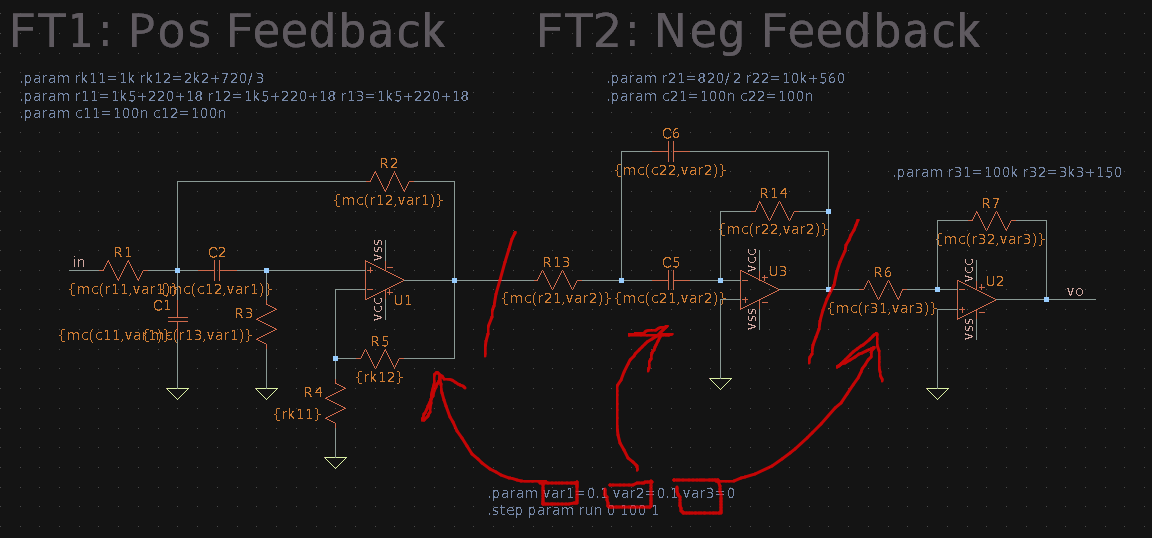
\includegraphics[scale=.35]{Secciones/Circ1/img/schMontecarlo.png}
    \caption{Analisis de montecarlo.}
    \label{prop}
\end{figure}

Utilizando Montecarlo se obtuvo una idea de que tanto podria distorsionarse la respuesta del filtro debido a la tolerancia de lo componentes. 

Por ultimo se utilizo la herramienta MEASURE para calcular el valor medio de la respuesta en la banda de paso para cada iteracion del analisis de Montecarlo, como adicional para tener una idea de en que rango de valores es mas probable que este la magnitud de la respuesta.

% --------------------------------------------------------------
\subsubsection{Realimentacion positiva (Sallen-Key)}

\noindent $>>$ \texttt{Para este caso se aplico el analisis de Montecarlo solo a la etapa de realimentacion positiva:}

\begin{figure}[H]
    \centering
    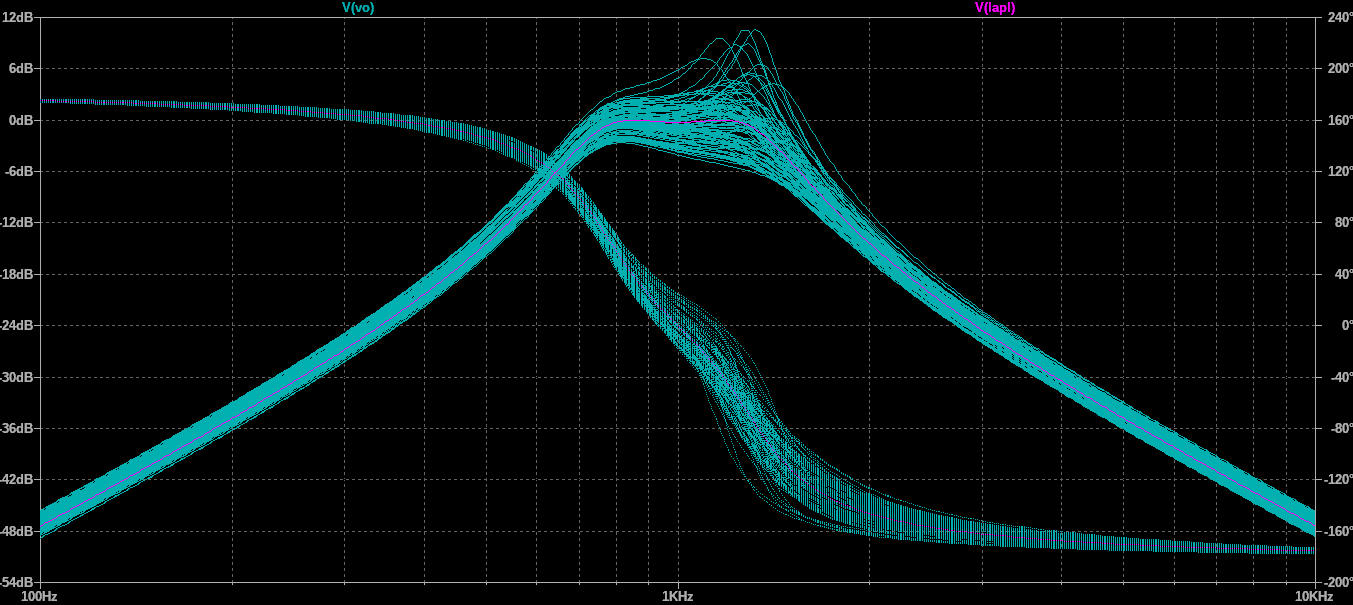
\includegraphics[scale=.3]{Secciones/Circ1/img/mtcarloPosVar.png}
    \caption{Montecarlo, primer etapa.}
    \label{prop}
\end{figure}

Se noto como variaciones en el valor de los componentes pueden generar un pico importante de casi 12dB en la magnitud de la respuesta a los 1.2kHz aprox. Vemos de esta forma como la primer etapa influye principalmente en la parte alta de nuestra banda de paso.

\subsubsection{Realimentacion negativa}

\noindent $>>$ \texttt{Para este caso se aplico el analisis de Montecarlo solo a la etapa de realimentacion negativa:}

\begin{figure}[H]
    \centering
    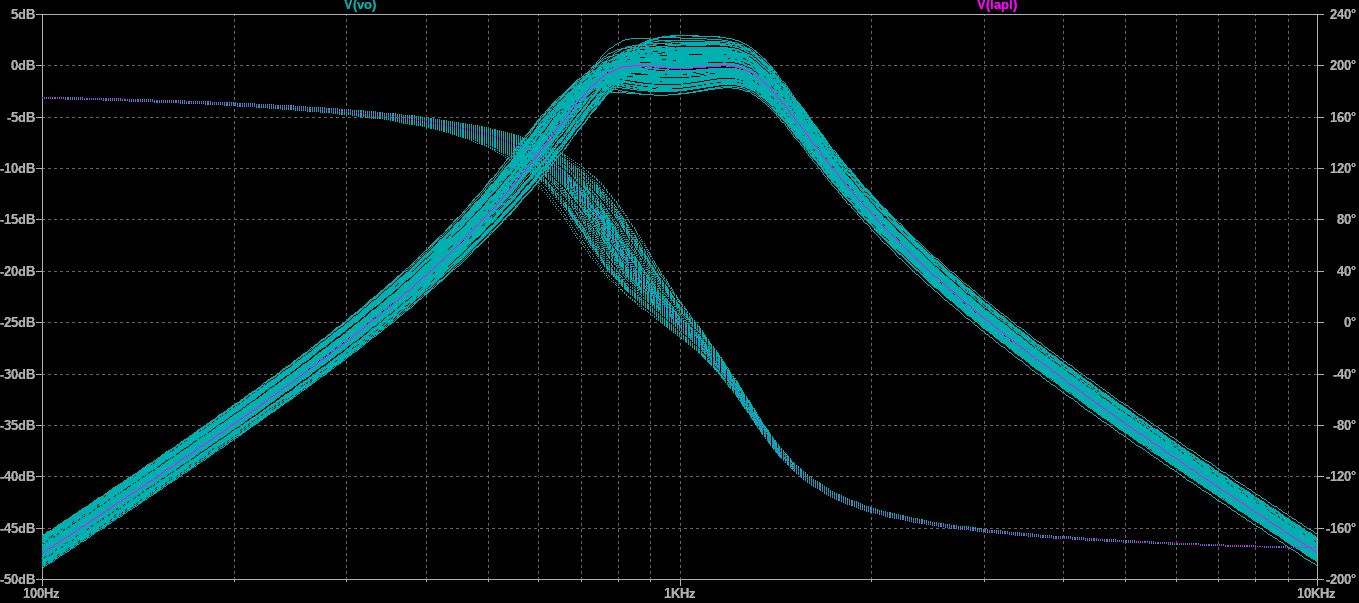
\includegraphics[scale=.3]{Secciones/Circ1/img/mtcarloNegVar.png}
    \caption{Montecarlo, segunda etapa.}
    \label{prop}
\end{figure}

Se noto como variaciones en el valor de los componentes generan un aumento en la magnitud a los 800Hz aprox. pero no genera picos abruptos de magnitud. Vemos de esta forma como la segunda etapa influye principalmente en la parte baja de nuestra banda de paso y en general la respuesta es mas suave, lo que puede deberse a la realimentacion negativa de esta topologia.

\subsubsection{Filtro final.}

\noindent $>>$ \texttt{Por ultimo se aplico el analisis de Montecarlo en ambas etapas considerando la tolerancia para todos los componentes del 10\%:}

\begin{figure}[H]
    \centering
    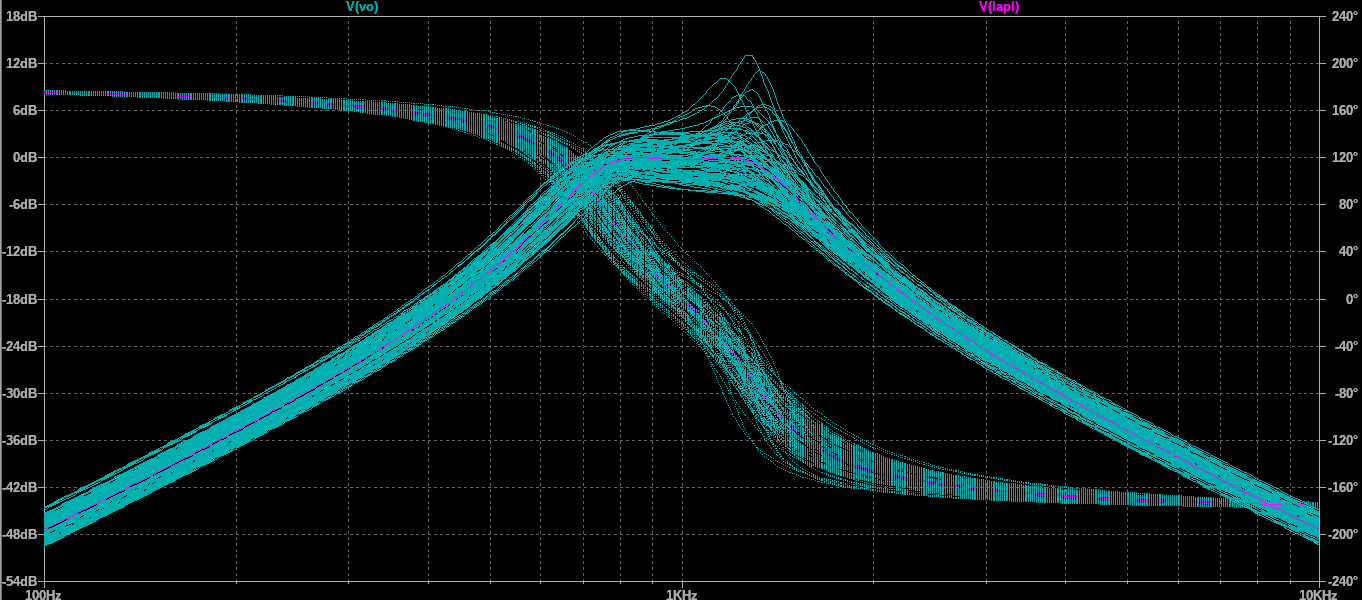
\includegraphics[scale=.3]{Secciones/Circ1/img/mtcarloFinal.png}
    \caption{Montecarlo, circuito final.}
    \label{prop}
\end{figure}

Con esto tenemos una idea de la respuesta del filtro para variaciones aleatorias en el valor de los componentes. \\

Ademas se utilizo la herramienta MEASURE por ejemplo para sacar el valor medio de la respuesta en la banda de paso para cada iteracion del analisis de Montecarlo.

\begin{figure}[H]
    \centering
    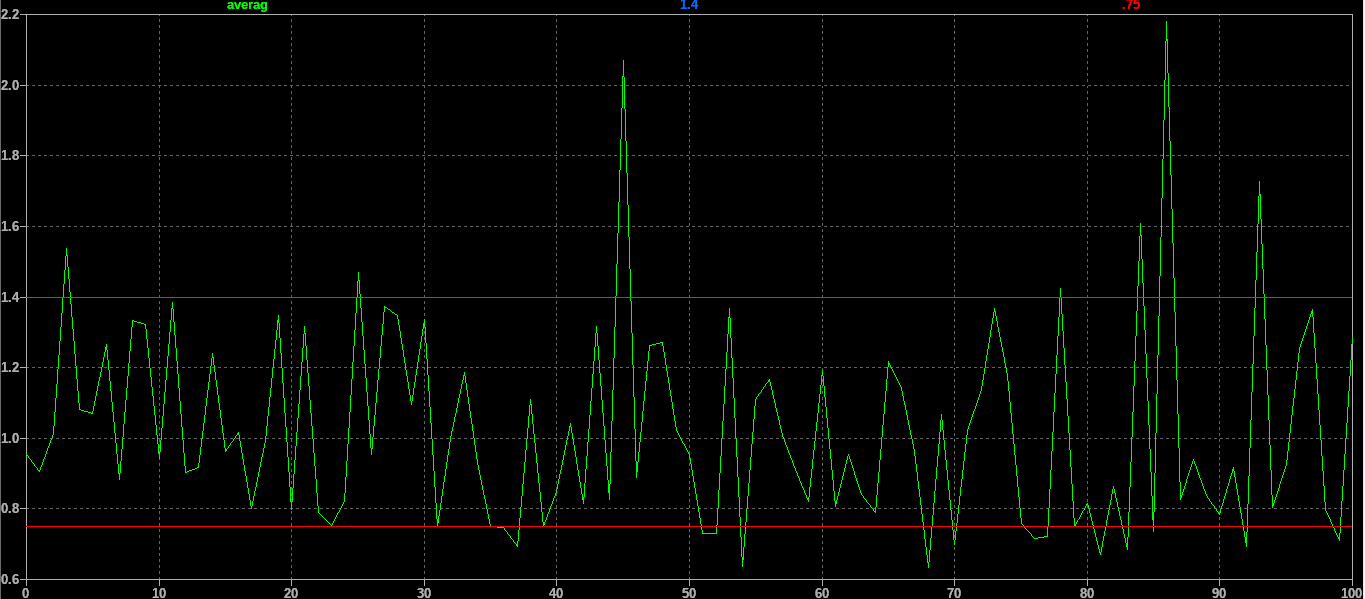
\includegraphics[scale=.3]{Secciones/Circ1/img/mtcarloAvg.png}
    \caption{Valores medios de magnitud en la banda de paso.}
    \label{prop}
\end{figure}

Con esto podemos darnos una idea aproximada de que el valor medio de la respuesta en la banda de paso esta comprendido entre los 0.75dB y 1.4dB la mayoria de las veces.

\paragraph{Mejorar respuesta}

Como se analizo antes, la distorsion mas grande de la respuesta es el pico de ganancia debido a la dispersion del valor de los componentes de la etapa con realimentacion positiva. Es claro que para mejorar la respuesta ante las posibles variaciones tenemos que mejorar los componentes de la primer etapa. \\

Teniendo en cuenta esto se realizo otro analisis pero con una tolerancia del 1\% en los componentes de la etapa con realimentacion positiva.

\begin{figure}[H]
    \centering
    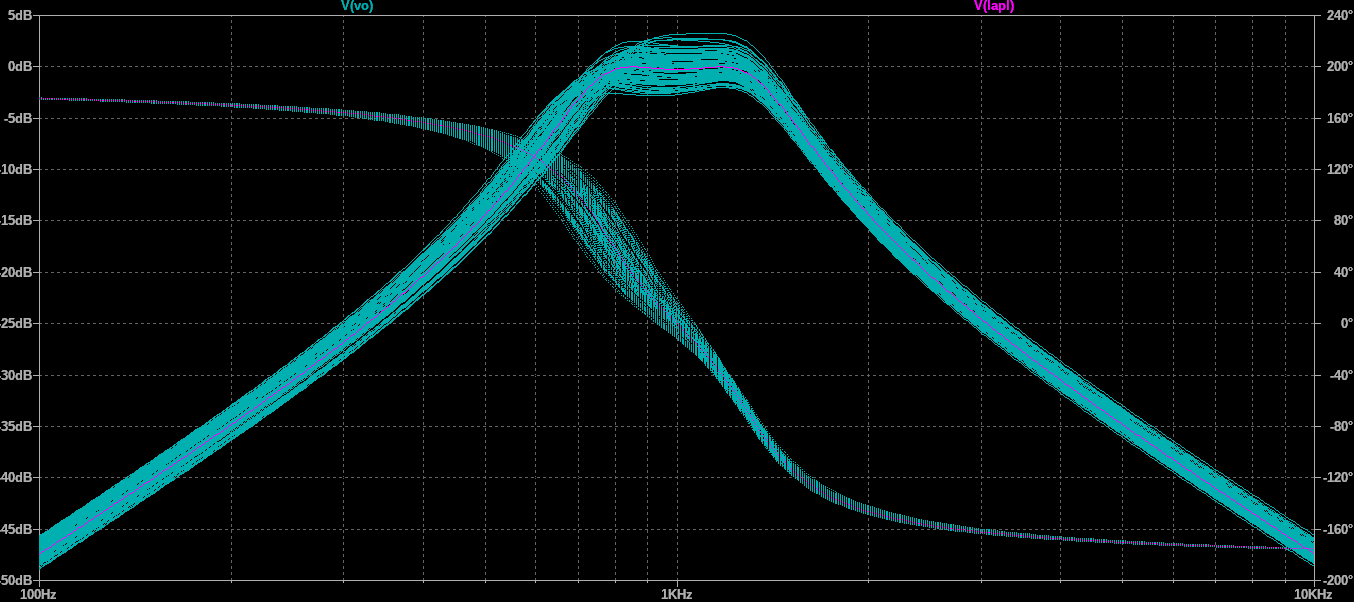
\includegraphics[scale=.3]{Secciones/Circ1/img/mtcarloMejorado.png}
    \caption{Primera etapa, componentes con tolerancia del 1\%.}
\end{figure}

Vemos como mejorando la tolerancia desaparece el pico de ganancia aumentando asi las probabilidades de sintetizar un filtro mas fiel a la respuesta requerida.